% This file was converted from HTML to LaTeX with
% gnuhtml2latex program
% (c) Tomasz Wegrzanowski <maniek@beer.com> 1999
% (c) Gunnar Wolf <gwolf@gwolf.org> 2005-2010
% Version : 0.4.
\section*{Scenegraph}
\subsection*{Einleitung}
Über den TCP port 3200 kann eine Server/Monitor Verbindung aufgebaut 
werden. Verbindet sich dann ein Monitor mit dem Server werden 
Informationen in folgender Reihenfolge übermittelt:

\begin{enumerate}
\item  (($<$EnvironmentInformation$>$)($<$SceneGraphHeader$>$)($<$SceneGraph$>$))
\item  (($<$GameState$>$)($<$SceneGraphHeader$>$)($<$SceneGraph$>$))
\item  (($<$partial GameState$>$)($<$SceneGraphHeader$>$)($<$partial/full SceneGraph$>$))
\end{enumerate}
Hinweis: Da für uns nur der Scene Graph Header und der Scene Graph an
 sich relevant sind, werden wir nicht näher auf 'EnviromentInformation' 
und 'GameState' eingehen.

\subsection*{Scene Graph Header}
Der Scene Graph Header sieht folgt aus:\\
\texttt{(Name Version Subversion)}

\begin{itemize}
\item  Name kann zwei werte annehmen:
\begin{itemize}
	\item  RSG steht für Ruby Scene Graph und zeigt an, dass es ein vollständig neuer Scene Graph ist.
	\item  RDS steht für Ruby Diff Scene und zeigt an, dass es ein 
	partieller Graph ist. Der partielle Scene Graph beinhaltet dann viele 
	leere Knoten und die aktualisierten Knoten.
\end{itemize}
\item  Version: Versions Nummer des Scene Graph.
\item  Subversion: Die Subversion Nummer des Scene Graph.
\end{itemize}
\subsection*{Scene Graph}
Der Scene Graph ist ein Baum, der aus verschiedenen Knoten besteht. 
Der root Knoten ist als $<$0;0;0$>$ definiert und hat keine Rotation. 
Die Position und Rotation eines jeden Kindes kann durch die 
Multplikation des root Knotens bis zum Kind herausgefunden werden.\\
Es werden aber keine spezifischen Objekte gespeichert, sondern nur Texturen der Objekte.

\subsubsection*{Base Knoten}
Jeder Knoten, der kein Transform Knoten, ein Static Mesh Knoten oder 
ein Light Knoten ist, ist ein Basis Knoten (inklusive des Root Knotens).
 Da er für uns irrelevant ist, gehen wir nicht näher auf den Knoten ein.

\begin{verbatim}(nd BN <contents>)
\end{verbatim}
\subsubsection*{Transform Knoten}
Transform Knoten sind 4x4 Transformationsmatrizen vom Aufbau:

\begin{verbatim}
[nx ox ax Px]
[ny oy ay Px]
[nz oz az Pz]
[ 0  0  0  1]
\end{verbatim}
wobei n, o, a für Normal, Orientierung und Annäherung stehen, die allesamt als Richtungsvektoren angegeben sind.\\
Die letzte Spalte ist ein Orstvektor, stellt also eine Position 
dar.
Wenn wir die Transform Knoten vom Root bis zu einem Kind multipliziert 
haben, enthalten die ersten drei Einträge der letzten Spalte demnach die
 Position des Kindes, das in dem Blatt gespeichert ist. Dies kann zum 
Beispiel ein Teil eines Naos oder der Ball sein.\\
Beispielnachricht:

\begin{verbatim}(nd TRF (SLT nx ny nz 0 ox oy oz 0 ax ay az 0 Px Py Pz 1 ))
\end{verbatim}
\subsubsection*{Geometry Nodes}
Die folgenden zwei Knoten definieren die Objekt Form. Sie spezifizieren ihre Maße und Texturen. Sie sind immer Blätter.

\paragraph*{StaticMesh}
Defniert die Textur, die aus der .obj Datei geladen wird:

\begin{verbatim}(nd StaticMesh (load <model>) (sSc <x> <y> <z>)
  (setVisible 1)
  (setTransparent)
  (resetMaterials <material-list>)
)
\end{verbatim}
model: Ist der Dateipfad zur .obj Datei.\\
sSc: Definiert die Maße des Objektes.\\
setVisible (optional): Gibt an, ob das Objekt sichtbar sein soll oder nicht.\\
setTransparent (optional): Unterschied zu setVisible unklar.\\
resetMaterials: Definiert eine Liste von Materialen, die mit der .obj Datei verknüpft sind.\\
\\
Beispielnachricht:

\begin{verbatim}(nd StaticMesh (load models/rlowerarm.obj) 
(sSc 0.05 0.05 0.05)(resetMaterials matLeft naowhite))
(nd StaticMesh (load models/naohead.obj) 
(sSc 0.1 0.1 0.1)(resetMaterials matLeft naoblack naogrey naowhite))
\end{verbatim}
\paragraph*{SMN}
\begin{verbatim}(nd SMN (load <type> <params>) (sSc <x> <y> <z>)
  (setVisible 1)
  (setTransparent)
  (sMat <material-name>)
)
\end{verbatim}
type:

\begin{itemize}
\item  StdUnitkBox
\item  StdUnitCylinder wobei $<$params$>$ zwei Angaben macht: Länge und Radius.
\item  StdUnitSphere
\item  StdCapsule with $<$params$>$ (Nicht benutzt in rcssserver3d 0.6.3; Parameter unklar) 
\end{itemize}
sSc: Definiert die Maße des Objektes.\\
setVisible (optional): Gibt an, ob das Objekt sichtbar sein soll oder nicht.\\
setTransparent (optional): Unterschied zu setVisible unklar.\\
sMat: Spezifiziert den Namen des Materials, das dem Objekt zugewiesen wird (z.B. matWhite, matYellow, etc.)\\
\\
Beispielnachricht:

\begin{verbatim}(nd SMN (load StdUnitBox) (sSc 1 31 1) (sMat matGrey))
(nd SMN (load StdUnitCylinder 0.015 0.08) (sSc 1 1 1) (sMat matDarkGrey))
\end{verbatim}
\subsubsection*{Light Node}
Ein Light Knoten zeigt an, wie Licht ein bestimmtes Objekt beeinflusst.

\begin{verbatim}(nd Light (setDiffuse x y z w) (setAmbient x y z w) (setSpecular x y z w))
\end{verbatim}
wobei $<$ x; y; z $>$ ein Vektor ist, der die Richtung des Lichtes definiert und w Skalenfaktor ist.\\
setDiffuse: Reflektion von unebenen Flächen.\\
setAmbient: Licht, das Objekte oder Szenerien umgibt.\\
setSpecular: Reflektion von glatten Oberflächen.

\subsection*{Beispielnachricht und Aufbau}
\begin{figure}[h]
\begin{center}
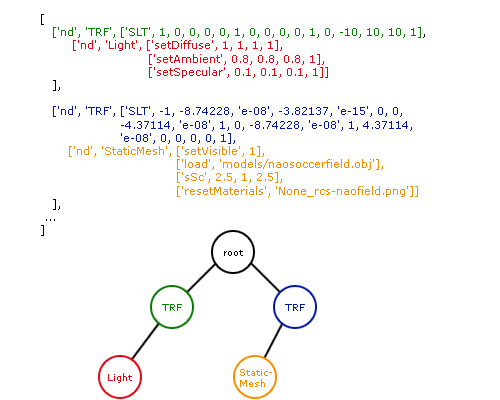
\includegraphics[scale=0.6]{Scene}
\end{center}
\caption{Graphische Veranschaulichung}
\end{figure}
Auszug aus einer Nachricht, die den kompletten Scene Graph enthält. 
Die Nachricht ist schon in der Form, in die sie der Parser bringt, also 
eine Liste und keine S-Expression mehr:

\begin{verbatim}[
   ['nd', 'TRF', ['SLT', 1, 0, 0, 0, 0, 1, 0, 0, 0, 0, 1, 0, -10, 10, 10, 1], 
        ['nd', 'Light', ['setDiffuse', 1, 1, 1, 1], ['setAmbient', 0.8, 0.8, 0.8, 1], ['setSpecular', 0.1, 0.1, 0.1, 1]]
   ],
   
   ['nd', 'TRF', ['SLT', -1, -8.74228, 'e-08', -3.82137, 'e-15', 0, 0, -4.37114, 'e-08', 1, 0, -8.74228, 'e-08', 1, 4.37114, 'e-08', 0, 0, 0, 0, 1], 
       ['nd', 'StaticMesh', ['setVisible', 1], ['load', 'models/naosoccerfield.obj'], ['sSc', 2.5, 1, 2.5], ['resetMaterials', 'None_rcs-naofield.png']]
   ],
 ...
]
\end{verbatim}
Abstrahieren wir die oben gezeigte Nachricht etwas um den Aufbau der Nachricht zu verstehen:

\begin{verbatim}[
   -$\,$- 1. Kind des root (Kind 1) -$\,$-
   ['nd', 'TRF', ['SLT', MATRIX], 
        -$\,$- 1. Kind von 'Kind 1' -$\,$-
        ['nd', 'Light', ['setDiffuse'], ['setAmbient'], ['setSpecular']]
   ],
   -$\,$- 2. Kind des root (Kind 2)-$\,$-
   ['nd', 'TRF', ['SLT', MATRIX], 
       -$\,$- 1. Kind von 'Kind 2' -$\,$-
       ['nd', 'StaticMesh', ['setVisible'], ['load'], ['sSc'], ['resetMaterials']]
   ],
...
]
\end{verbatim}
Der Vollständigkeit halber hier eine (partielle) Beispielnachricht eines aktualisierten Baumes:

\begin{verbatim}[
    ['nd', 
        ['nd']], 
    ['nd', 
        ['nd']], 
    ['nd', 
        ['nd', 'StaticMesh']
...
]
\end{verbatim}
\subsection*{Implementierung}
\subsubsection*{Datenstrukturen}
Um alle Knoten zu speichern, haben wir für jeden Knoten eine Datenstruktur angelegt.

\subsubsection*{Wichtigsten Methoden}
def run\_cycle(self): Wird vom Agenten aufgerufen, um dann seine 
Position zu bestimmen. Hier wird der Header überprüft und es wird 
entweder ein komplett neuer Graph eingelesen oder ein vorhandener wird 
aktualisiert.\\
def create\_trans\_node(self,msg): Erstellt ein Transform Knoten und speichert die Matrix als numpy Matrix.

\begin{verbatim}  Scenegraph Matrix: [SLT, nx, ny, nz, 0, ox, oy, oz, 0, ax, ay, az, 0, Px, Py, Pz, 1]
 
  numpy Matrix:
  ( ((nx, ox, az, Px]),
     (ny, oy, ay, Py),
     (nz, oz, az, Pz),
     (0 ,  0,  0,  1)) )
    
\end{verbatim}
def create\_light\_node(self,msg): Erstellt einen Light Knoten. 
Speichere dabei den diffuse-, ambient- und specular-Inhalt jeweils als 
numpy Array.\\
def create\_smn\_node(self,msg): Erstellt einen SMN Knoten. Die sSc- und load-Inhalte werden als Listen gespeichert.\\
def create\_static\_mesh\_node(self,msg): Erstellt einen SMN Knoten.
 Die sSc-, reset- und load-Inhalte werden als Listen gespeichert.\\
def update\_scene(self, msg): Aktualisiert einen vorhandenen Scenegraph.\\
def get\_position(self, team, naoID): Gibt die aufsummierte Matrix
 vom Root bis zum NAO zurück. Als Parameter werden das Team (left,right)
 und die Rückennummer des NAOs benötigt.\\
def get\_position\_xy(self, team, naoID): Gibt die x,y-Position des
 NAOs zurück. Als Parameter werden das Team (left,right) und die 
Rückennummer des NAOs benötigt.\\
def get\_ball\_position(self): Gibt die x,y-Position des Balles zurück.
